\section{PyTorch Objects}
\subsection{Tensor}

What it means to represent and organize data in a \textit{tensor} can be viewed for \gls{ML} as two different concepts.
\begin{description}
	\item[Data Storage] Multidimensional Arrays/data tensor. Note: Arrays are not matrices. For example, a scalar is zero-dimensional, a vector is one-dimensional, a matrix is two-dimensional, and so on. This concept is used to store data, depending on the relationship.
	\item[Multilinear Mapping (Mathematical object)] This may express a multilinear relationship between a set of algebraic objects.
\end{description}
The data tensor may be analyzed or preprocessed either by tensor methods, which rely on tensor methods like decomposition that are rooted in the understanding of tensors as multilinear mapping. Through \gls{AI_NN}, these data tensors or preprocessed data tensors can be further analyzed.\\
% See https://tspace.library.utoronto.ca/bitstream/1807/65327/11/Vasilescu_M_Alex_O_200911_PhD_thesis.pdf#page44
% See https://en.wikipedia.org/wiki/Tensor_(machine_learning)

In \textit{PyTorch} a \textit{tensor} is data abstraction, aka data tensor. The relevant module for this is $\verb|torch|$. By using $\verb|torch.empty(3,4)|$ a tensor has 3 expression for the first dimension and 4 for the second dimension. Note: $\verb|torch.empty(1)| $ creates a tensor equal to a scalar object. $\verb|torch.empty(3)|$  a vector and $\verb|torch.empty(2,2)|$ a matrix, and $\verb|torch.empty(3,3,3)|$ a higher dimensional object.


\subsection{nn.Linear}

This module is fundamental in PyTorch, not only for \gls{AI_NN}. The $\verb|nn.Linear|$ is a linear layer, that applies a lineare transformation to input data using \textit{weights} and \textit{biases}.\\

This module find versatial application

\begin{itemize}
	\item \textbf{FFNN} This kind of networks are fully connected with at lest three layers. The module $\verb|nn.linear|$ is used to implement this connection.
	\item \textbf{Linear Regression} In this case the module can be used to model the linear implementation of the equation.
	\item \textbf{Data Transformation} In case the data need to be transformed into higher dimenension, then his module can help
	\item \textbf{Further deep learning architecture} For example modules like Autoencoder using this module as well. 
\end{itemize}

Related topics: Comparing $\verb+nn.Linear+$ to $\verb+nn.Conv2d+$ 
while $\verb+ nn.Linear+$ applies a linear transformation the $\verb+nn.Conv2d+$ a 2D convulation. 
% https://docs.kanaries.net/topics/Python/nn-linear

As explained in the previous section the implementation of a lineare transformation looks like

\begin{lstlisting}[language=iPython]
	import torch
	from torch import nn
	
	# Create a dataset with 3 featrures (x_input_dataset_1, x_input_dataset_2, x_input_dataset_3) and 1000 samples.
	# Each sample is a vector of 3 features.
	x_input_dataset_input_dataset = torch.randn(100,3) # create a input dataset
	
	# The nn.Linear layer performs two main tasks:
	# 1. Initializes the weight matrix_input_dataset $W$ and bias vector $b$.
	# 2. Applies the affine transformation $\vec{y} = \vec{x_input_dataset} W^T + \vec{b}$ to the input data $\vec{x_input_dataset}$.
	#    Here, $\vec{x_input_dataset}$ is the input tensor, $W$ is the weight matrix_input_dataset, and $b$ is the bias vector.
	hidden_hidden_layer_1 = nn.Linear(
	in_features=3,  # Number of input features ($x_input_dataset_1$, $x_input_dataset_2$, $x_input_dataset_3$), not the dataset size.
	out_features=4  # Number of output features ($y_1$, $y_2$, $y_3$, $y_4$), i.e., neurons in this layer.
	)
	
	# Pass the input tensor $\vec{x_input_dataset}$ (1000 datasets by 3 features) through the linear layer.
	# This computes the output $\vec{y} = \vec{x_input_dataset} W^T + \vec{b}$,
	y_1 = hidden_hidden_layer_1(
	x_input_dataset_input_dataset
	)
\end{lstlisting}



\section{Linear Transformation for Two Layer} 
\paragraph{Weight Matrix}
Each node $n^{(j)}_i$ in layer $j$ has an output $y^{(j)}_i$, where 
\begin{itemize}
	\item[$j$] Index for the layer,
	\item[$i$] Index for the node in layer $j$,
	\item[$y$] Output of node $i$ in layer $j$.
\end{itemize}

In the example, layer 1 has four nodes, therefore the outputs are
\begin{align}
	y^{(1)}_1, \dots, y^{(1)}_4.
\end{align}

\begin{figure}[H]
	\centering
	\scalebox{0.6}{%
		
		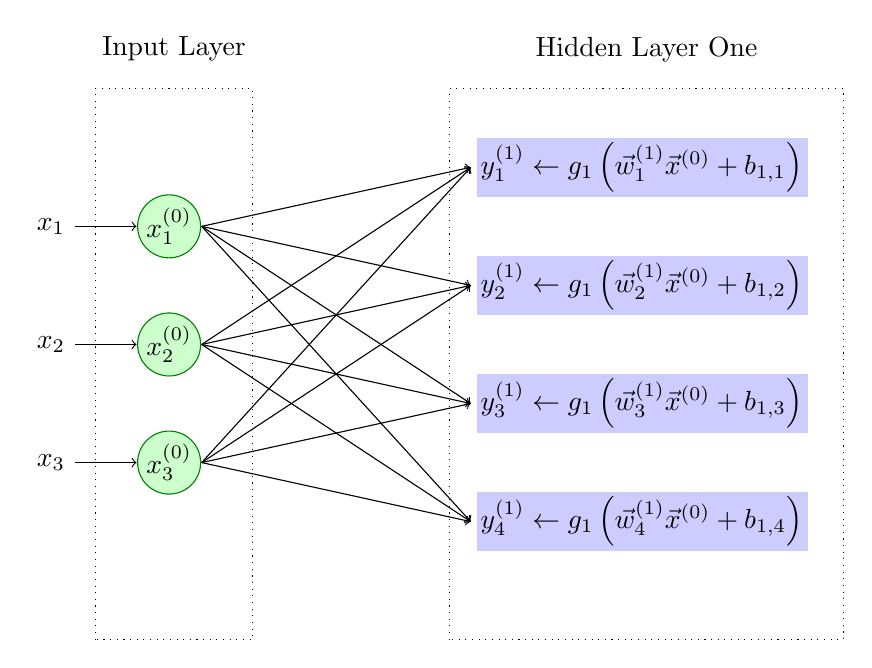
\begin{tikzpicture}
			
			% Drawing input on the left side each input layer
			\def\movefactorZeroZeroCircles{-7.5}
			\foreach \x/\layerindex in {1/x}{
				\foreach \y/\neuroindex in {7/1,5/2, 3/3}{
					\node[name=\layerindex_\neuroindex] at (\x*3.25 +\movefactorZeroZeroCircles -0.8125,\y*0.75) {% function desciption
						$x_\neuroindex$
					};
					
				}
			}
			
			% Input layer with two neurons
			\draw[dotted] (-4.5,0) rectangle ++(2,7);
			\node at (-3.5,7.5) {Input Layer}; % Label for the Hidden layer one
			
			% Drawing circles on the left side of the Hidden layer one
			\def\movefactorZeroCircles{-6}
			\foreach \x/\layerindex in {1/0}{
				\foreach \y/\neuroindex in {7/1,5/2, 3/3}{
					\filldraw[fill=green!20, draw=green!50!black] (\x*3.25 +\movefactorZeroCircles -0.8125,\y*0.75) circle circle (0.4);
					\node[name=\layerindex_\neuroindex] at (\x*3.25 +\movefactorZeroCircles -0.8125,\y*0.75) {% function desciption
						$x^{(\layerindex)}_{\neuroindex}$
					};
				}
			}   
			
			% Hidden layer one with four neurons
			\draw[dotted] (0,0) rectangle ++(5,7);
			\node at (2.5,7.5) {Hidden Layer One}; % Label for the Hidden layer one
			
			% Drawing neurons and displaying function in the Hidden layer one
			\foreach \x/\layerindex in {1/1}{
				\def\forwardedlayerindex{0}
				\foreach \y/\neuroindex in {8/1,6/2,4/3,2/4}{
					\fill[blue!20] (\x*3.25 -2.9,\y*0.75-0.375) rectangle ++(4.2,0.75);
					\node[name=\layerindex_\neuroindex] at (\x*3.25-0.8125,\y*0.75-0.375+0.375) {% function desciption
						$y_\neuroindex^{(\layerindex)} \leftarrow g_\layerindex \left(\vec{w}^{(\layerindex)}_{\neuroindex}\vec{x}^{(\forwardedlayerindex)}+b_{\layerindex,\neuroindex}\right)$
					};
				}
			}
			
			
			
			% Arrows connecting right side of input to left side of the corresponding cicle
			\draw[->] (x_1) -- (0_1);
			\draw[->] (x_2) -- (0_2);
			\draw[->] (x_3) -- (0_3);
			
			
			% Arrows connecting right side of circels to left side of the corresponding inner box of the Hidden layer one
			\foreach \x in {1,2,3}
			\foreach \y in {1,2,3,4}
			\draw[->] (0_\x.east) -- (1_\y.west);
			
			
		\end{tikzpicture}
		
	}
	\caption{Example Two Layer Network}
\end{figure}

In a \gls{FFNN}, all outputs of the previous layer are connected to the next layer. Hence, each node $i$ requires a weight vector
\begin{align}
	w^{(j)}_i = \begin{bmatrix} w^{(j)}_{i, 1} & \dots & w^{(j)}_{i, k} \end{bmatrix}^T,
\end{align}
where $k$ is the index for the output of the previous layer. In this example, the input layer has 3 nodes, and therefore three outputs:
\begin{align}
	y^{(0)}_1, y^{(0)}_2, y^{(0)}_3.
\end{align}
For the whole layer $1$, the weights may be represented in a tensor:
\begin{align}
 \begin{bmatrix} w_1^{(1)} & w_2^{(1)} & w_3^{(1)} & w_4^{(1)} \end{bmatrix}^T
\end{align}
which can be represented as a matrix:
\begin{align}
	\begin{pmatrix}
		w^{(j)}_{1, 1} & \dots & w^{(j)}_{n, 1} \\
		\vdots & \ddots & \vdots \\ 
		w^{(j)}_{1, m} & \dots & w^{(j)}_{n, m}
	\end{pmatrix}^T \rightarrow
	\begin{pmatrix}
		w^{(1)}_{1, 1} & w^{(1)}_{2, 1} & w^{(1)}_{3, 1} & w^{(1)}_{4, 1} \\
		w^{(1)}_{1, 2} & w^{(1)}_{2, 2} & w^{(1)}_{3, 2} & w^{(1)}_{4, 2} \\
		w^{(1)}_{1, 3} & w^{(1)}_{2, 3} & w^{(1)}_{3, 3} & w^{(1)}_{4, 3}  
	\end{pmatrix}^T
\end{align}

\paragraph{Transformation of the whole dataset}

The object \verb+nn.Linear+ handles multiple rows of input data, i.e., a batch. Although architecture diagrams of a \gls{AI_NN} often illustrate the flow for a \emph{single input sample}, in practice, training is done with batches of data.

When creating a layer with \verb+nn.Linear(in_features, out_features)+, the object internally initializes:
\begin{itemize}
	\item a weight matrix $A \in \mathbb{R}^{\text{out\_features} \times \text{in\_features}}$,
	\item a bias vector $b \in \mathbb{R}^{\text{out\_features}}$.
\end{itemize}

Given an input batch $x \in \mathbb{R}^{B \times n}$, where $B$ is the batch size and $n$ is the number of input features, the transformation performed by the layer is:
\begin{align}
	y = x A^T + b
\end{align}

Here:
\begin{itemize}
	\item $x \in \mathbb{R}^{B \times n}$ is the input matrix (batch of $B$ samples, each with $n$ features),
	\item $A \in \mathbb{R}^{m \times n}$ is the weight matrix (for a layer with $m$ output neurons),
	\item $A^T \in \mathbb{R}^{n \times m}$ is the transposed weight matrix,
	\item $b \in \mathbb{R}^{m}$ is the bias vector (broadcasted across the batch),
	\item $y \in \mathbb{R}^{B \times m}$ is the output matrix, where each row contains the raw scores (logits) for one sample.
\end{itemize}

Let:
\begin{itemize}
	\item each input sample have $n = 3$ features,
	\item the batch size be $B = 5$ (i.e., 5 samples at once),
	\item the next layer have $m = 4$ neurons (e.g., hidden layer),
\end{itemize}

Then:
\begin{align*}
	x &\in \mathbb{R}^{5 \times 3}, \\
	A &\in \mathbb{R}^{4 \times 3}, \quad A^T \in \mathbb{R}^{3 \times 4}, \\
	b &\in \mathbb{R}^{4}, \\
	y &= x A^T + b \in \mathbb{R}^{5 \times 4}.
\end{align*}

Let
\begin{align} 
	x = \begin{pmatrix}
		1 & 2 & 3 
	\end{pmatrix}
	\text{ and }
	A^T = \begin{pmatrix}
		0.1 & 0.2 & 0.3 & 0.4 \\
		0.5 & 0.6 & 0.7 & 0.8 \\
		0.9 & 1.0 & 1.1 & 1.2 \\
	\end{pmatrix}\text{ and } b= \begin{pmatrix}
		0.899 & 0.6564 & 0.2342 & 0.2823
	\end{pmatrix}
\end{align}

Then the product matrix $y = x \cdot A^T + b$ is given by:


\begin{align}
	y = \begin{pmatrix}
		1 & 2 & 3 
	\end{pmatrix} \cdot \begin{pmatrix}
		0.1 & 0.2 & 0.3 & 0.4 \\
		0.5 & 0.6 & 0.7 & 0.8 \\
		0.9 & 1.0 & 1.1 & 1.2 \\
	\end{pmatrix} + \begin{pmatrix}
		0.899 & 0.6564 & 0.2342 & 0.2823
	\end{pmatrix}
\end{align}

The resulting matrix $y$ obtained:

\begin{align}
	y = \begin{pmatrix}
		3.8 & 4.4 & 5.0 & 5.6 
	\end{pmatrix} = \begin{bmatrix}
		y^{(1)}_1, y^{(1)}_2,  y^{(1)}_3, y^{(1)}_4
	\end{bmatrix}.
\end{align}

Lets considering matrix $x$ as the \textbf{input matrix} with  $m=5$ rows of data and $n=3$.\\

Let
\begin{align} 
	x = \begin{pmatrix}
		1 & 2 & 3 \\
		4 & 5 & 6 \\
		7 & 8 & 9 \\
		10 & 11 & 12 \\
		13 & 14 & 15 \\
	\end{pmatrix}
	\text{ and }
	A^T = \begin{pmatrix}
		0.1 & 0.2 & 0.3 & 0.4 \\
		0.5 & 0.6 & 0.7 & 0.8 \\
		0.9 & 1.0 & 1.1 & 1.2 \\
	\end{pmatrix}\text{ and } b= \begin{pmatrix}
		0.899 & 0.6564 & 0.2342 & 0.2823\\
		0.899 & 0.6564 & 0.2342 & 0.2823\\
		0.899 & 0.6564 & 0.2342 & 0.2823\\
		0.899 & 0.6564 & 0.2342 & 0.2823\\
		0.899 & 0.6564 & 0.2342 & 0.2823\\
	\end{pmatrix}
\end{align}
Note, each row in the vector of the bias $b$ represents the \textbf{outputfeature} size and therefore the number of nodes in the forward connected layer. 
Then the product matrix $y = x \cdot A^T + b$ is given by:


\begin{align}
	y = \begin{pmatrix}
		1 & 2 & 3 \\
		4 & 5 & 6 \\
		7 & 8 & 9 \\
		10 & 11 & 12 \\
		13 & 14 & 15 \\
	\end{pmatrix} \cdot \begin{pmatrix}
		0.1 & 0.2 & 0.3 & 0.4 \\
		0.5 & 0.6 & 0.7 & 0.8 \\
		0.9 & 1.0 & 1.1 & 1.2 \\
	\end{pmatrix} + \begin{pmatrix}
		0.899 & 0.6564 & 0.2342 & 0.2823\\
		0.899 & 0.6564 & 0.2342 & 0.2823\\
		0.899 & 0.6564 & 0.2342 & 0.2823\\
		0.899 & 0.6564 & 0.2342 & 0.2823\\
		0.899 & 0.6564 & 0.2342 & 0.2823\\
	\end{pmatrix}
\end{align}

The resulting matrix $y$ obtained:

\begin{align}
	y = \begin{pmatrix}
		3.8 & 4.4 & 5.0 & 5.6 \\
		9.1 & 10.6 & 12.1 & 13.6 \\
		14.4 & 17.2 & 20.0 & 22.8 \\
		19.7 & 23.8 & 27.9 & 32.0 \\
		25.0 & 30.4 & 35.8 & 41.2 \\
	\end{pmatrix} = \begin{bmatrix}
		y^{(1)}_1, y^{(1)}_2,  y^{(1)}_3, y^{(1)}_4
	\end{bmatrix}.
\end{align}

This represents the resulting matrix after performing the matrix multiplication $y = x \cdot A +b$, where each row is a dataset and each column the outputvalue of outputlayer nodes.\\

\section{Implementation of a Multilayer Perceptron (MLP) in PyTorch}

\paragraph{Code Overview}
The following code implements a \gls{AI_NN}, more specifically a \textbf{Multilayer Perceptron (MLP)}, using the PyTorch framework. The network is constructed as a sequence of fully connected layers (also known as \textit{dense layers}) and uses activation functions to introduce non-linearity.

\paragraph{Network Architecture}
The implemented neural network consists of:
\begin{itemize}
	\item An \textbf{input layer} with $n=4$ features
	\item \textbf{Two hidden layers} with $5$ and $3$ neurons respectively
	\item An \textbf{output layer} with $5$ output nodes (interpretable as categories or regression outputs)
\end{itemize}

Each layer is represented as an affine transformation:
\begin{align}
	z^{(l)} &= w^{(l)} x^{(l)} + b^{(l)}
\end{align}
followed by a nonlinear \textbf{activation function}:
\begin{align}
	y^{(l)} &= \phi\left(z^{(l)}\right)
\end{align}

The ReLU activation function $\phi(z) = \max(0, z)$ is used for the hidden layers, and a sigmoid activation function $\sigma(z) = \frac{1}{1+e^{-z}}$ is applied at the output layer.

\paragraph{Forward Pass}
The \texttt{forward} method of the class \texttt{FFNN} defines the data flow through the network:
\begin{enumerate}
	\item Input data $x \in \mathbb{R}^{100 \times 4}$ is passed to the network (100 samples with 4 features each)
	\item The data is transformed sequentially by each layer and activation function
	\item The final output $y \in \mathbb{R}^{100 \times 5}$ represents the predicted values for each sample
\end{enumerate}

\paragraph{Code Instantiation}
The network is instantiated with the following code:
\begin{lstlisting}[language=iPython]
	NN_1 = FFNN(4, 5, 3, 5)
	input_data = torch.randn(100, 4)
	# Pass the input data through the network. PyTorch calls the forward methode
	FFNN_output = NN_1(input_data)
\end{lstlisting}

\paragraph{Interpretation}
This model serves as a basic but functional example of how a \textbf{feedforward neural network} (FFNN) operates. It can be adapted for classification or regression tasks by changing the output activation and loss function accordingly. The structure mimics the conceptual \textit{layered perceptron model} introduced earlier in 



\begin{lstlisting}[language=iPython]
	import torch
	from torch import nn
	import torch.nn.functional as F
	
	class FFNN(nn.Module):
	def __init__(self, input_feature_size, layer_one_nodes, layer_two_nodes, output_category):
	super(FFNN, self).__init__()
	self.hL1 = nn.Linear(input_feature_size, layer_one_nodes)
	self.hL2 = nn.Linear(layer_one_nodes, layer_two_nodes)
	self.hL3 = nn.Linear(layer_two_nodes, output_category)
	
	def forward(self, x_input_dataset):
	y_layer = F.relu(self.hL1(x_input_dataset))
	y_layer = F.relu(self.hL2(y_layer))
	y_layer = F.sigmoid(self.hL3(y_layer))
	return y_layer
	
	# Create an instance of the network
	ds_feature_size = 4
	hidden_layer_one_size = 5
	hidden_layer_two_size = 3
	ds_target_size = 5
	
	NN_1 = FFNN(ds_feature_size, hidden_layer_one_size, hidden_layer_two_size, ds_target_size)
	
	print("Architecture of instance of the fully connected neural network: ", NN_1)
\end{lstlisting}

\section{Training and Evaluating the model}
To train a model, we must 
\begin{itemize}
	\item define a loss function to calculate the gradient, in order to know, who the diviate of the target value is evaluated.
	\item and an optimizer, that updates the parameter for each round.
\end{itemize}

For the loss function the \textit{binary crossentropy} function is selected, which measures a criterion between the target value and the input probability. And for the optimizer we use \textit{storchastic gradient descent}.\\



\begin{lstlisting}[language=iPython, caption={}]
	
	# Setting up loss and optimizer
	loss_fn = nn.BCELoss()
	
	learning_rate = 0.1
	optimizer = torch.optim.SGD(NN_1.parameter(), lr= learning_rate)
	
	# Setting up training runs
	num_epochs = 100
	loss_values = []
	
	
	for epoch in range(num_epochs):
	for X, y in train_dataloader:
	# zero the parameter gradients
	optimizer.zero_grad()
	
	# forward + backward + optimize
	pred = model(X)
	loss = loss_fn(pred, y.unsqueeze(-1))
	loss_values.append(loss.item())
	loss.backward()
	optimizer.step()
	
	print("Training Complete")
	
	"""
	
	
\end{lstlisting}
